\section{AIT and Kolmogorov complexity}
%%%%%%%%%%%%%%%%%%%%%%%%%%%%%%%%%%%%%%%%%%%%%%%%%%%%%%%%%%%%%%%%%%%%%%
\begin{frame}[label=intro3]{Kolmogorov complexity ($\Ko$) I}
 We can think of agents as physical systems, and in turn,  of physical systems as dynamical systems calculating (effectively computable) functions.   This allows us to analyze agents from the standpoint of computation theory.
 \begin{alertblock}{Warning: Computation is a mathematical concept (Turing machine)}
The use of computational framework  in KT should not be construed to mean that the brain is literally a physical von Neumann computer (such as a laptop).
\end{alertblock}\vfill 
 
A computational perspective  leads us directly into algorithmic information theory (AIT) and its central concept: 


\begin{definition}[Kolmogorov complexity  of a dataset $\Ko$]
The length of the shortest program capable of generating  the dataset \citep{Kolomgorov1965,Cover:2006aa}.  
\end{definition} \vfill

\end{frame}


%%%%%%%%%%%%%%%%%%%%%%%%%%%%%%%%%%%%%%%%%%%%%%%%%%%%%%%%%%%%%%%%%%%%%%
\begin{frame}[label=intro3]{Kolmogorov complexity ($\Ko$) II}
 \begin{center}%\includegraphics[height=1.2cm]{COPL}%
  %\hspace{2cm}
  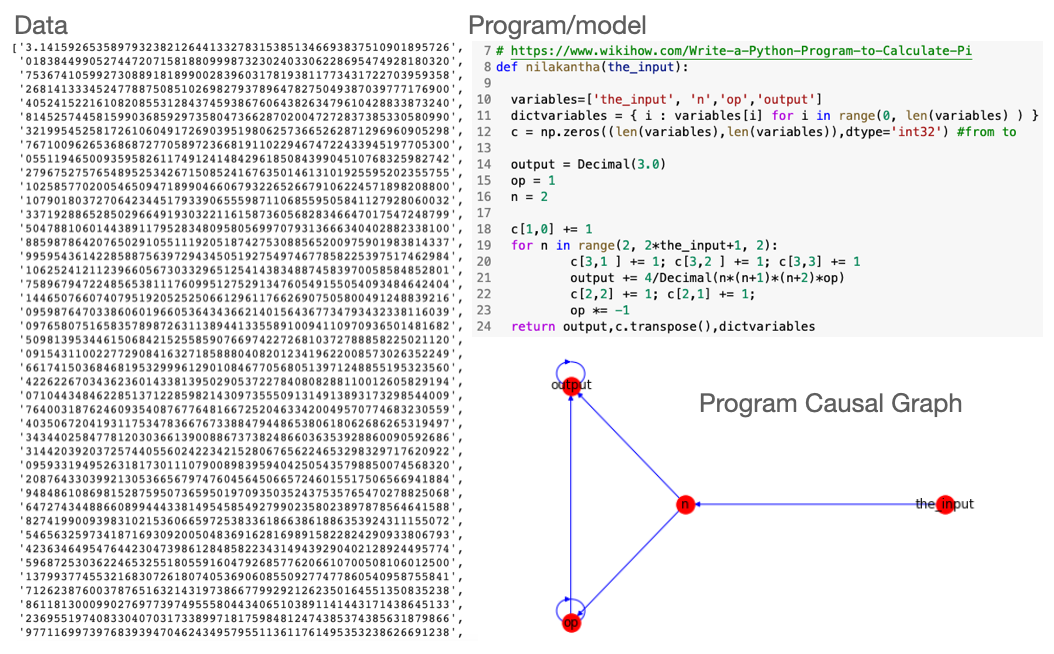
\includegraphics[height=7.2cm]{img/pi.png}
  \end{center}
\end{frame}

%%%%%%%%%%%%%%%%%%%%%%%%%%%%%%%%%%%%%%%%%%%%%%%%%%%%%%%%%%%%%%%%%%%%%%
% \begin{frame}[label=intro3]{Mutual algorithmic information ($\mathcal M$)}
% With 
% \K at hand, we can define an algorithmic version of mutual information we will also need: \vfill

% \begin{definition}[Mutual algorithmic information complexity  $\mathcal M$]
% The {\em mutual algorithmic information  $\mathcal M(x:y)$ between two strings $x$ and $y$, is given by  }
% $$
% \mathcal M(x \!:\!y) = \Ko(x) +\Ko(y)- \Ko(x,y)
% $$
% %where $\Ko(y|x)$ is the complexity of the string $y$ if the computer has access to $x$ 
% \citep{Li:1997aa, Grunwald:2004aa}.  
% \end{definition}
% \end{frame}

%%%%%%%%%%%%%%%%%%%%%%%%%%%%%%%%%%%%%%%%%%%%%%%%%%%%%%%%%%%%%%%%%%%%%%
% \begin{frame}[label=ladila]{Hierarchy class \citep{Fitch2014}}
% Not all programming languages are equal. Recurrence is needed for Turing completeness, for example. 
%  \begin{center}%\includegraphics[height=1.2cm]{COPL}%
%   %\hspace{2cm}
%   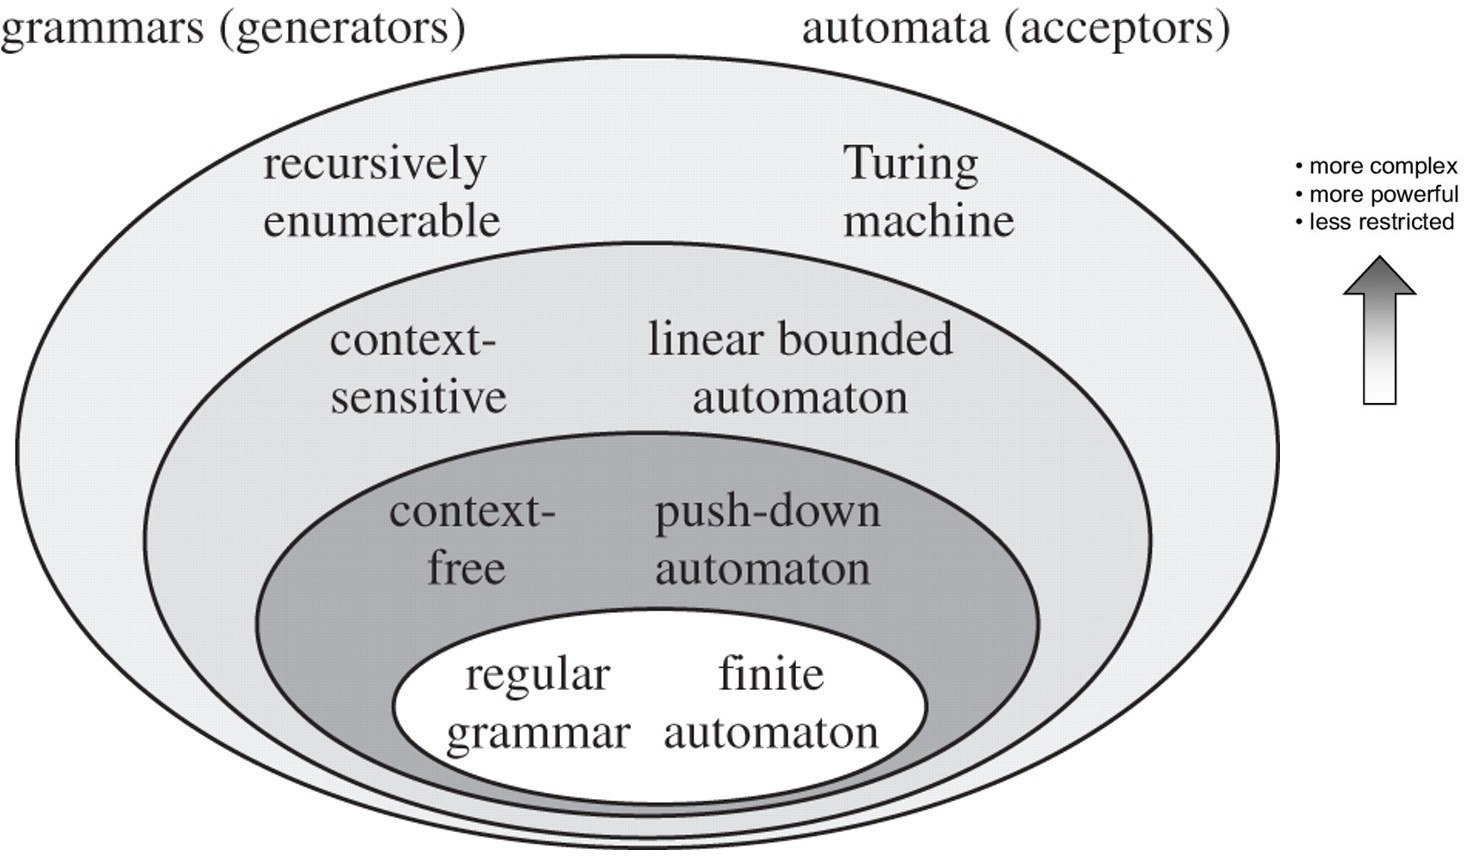
\includegraphics[height=5.5cm]{img/chomsky.jpg}
%   \end{center}
% \end{frame}

%%%%%%%%%%%%%%%%%%%%%%%%%%%%%%%%%%%%%%%%%%%%%%%%%%%%%%%%%%%%%%%%%%%%%%
\begin{frame}[label=ladila]{Model I}
The notion of {\bf model} is central in KT and other theories of consciousness. \vfill

 %With AIT as a basis, we can now define what a  model is and an optimal model. \vfill 
 
 \begin{definition}[Model]
 A  model of a dataset is any program that generates the dataset. 
 \end{definition}
Models may differ in two ways: they may implement different functions, or they may implement the same function in different ways. Both aspects matter here.  We focus on those that implement the right functions succinctly. \vfill 
 
\begin{definition}[Optimal model]
The optimal model of a dataset is the shortest program that generates (or, equivalently, compresses) the dataset.
\end{definition}
\end{frame}


%%%%%%%%%%%%%%%%%%%%%%%%%%%%%%%%%%%%%%%%%%%%%%%%%%%%%%%%%%%%%%%%%%%%%%
\begin{frame}[label=ladila]{Model II}

An {\bf optimal model needs to capture and exploit all the structure in the dataset}---and nothing else. In some sense, the {\em structure of the model can be described by the group of symmetries of the dataset}  \citep{Ruffini:2016ad}. 
 \begin{center}%\includegraphics[height=1.2cm]{COPL}%
  %\hspace{2cm}
  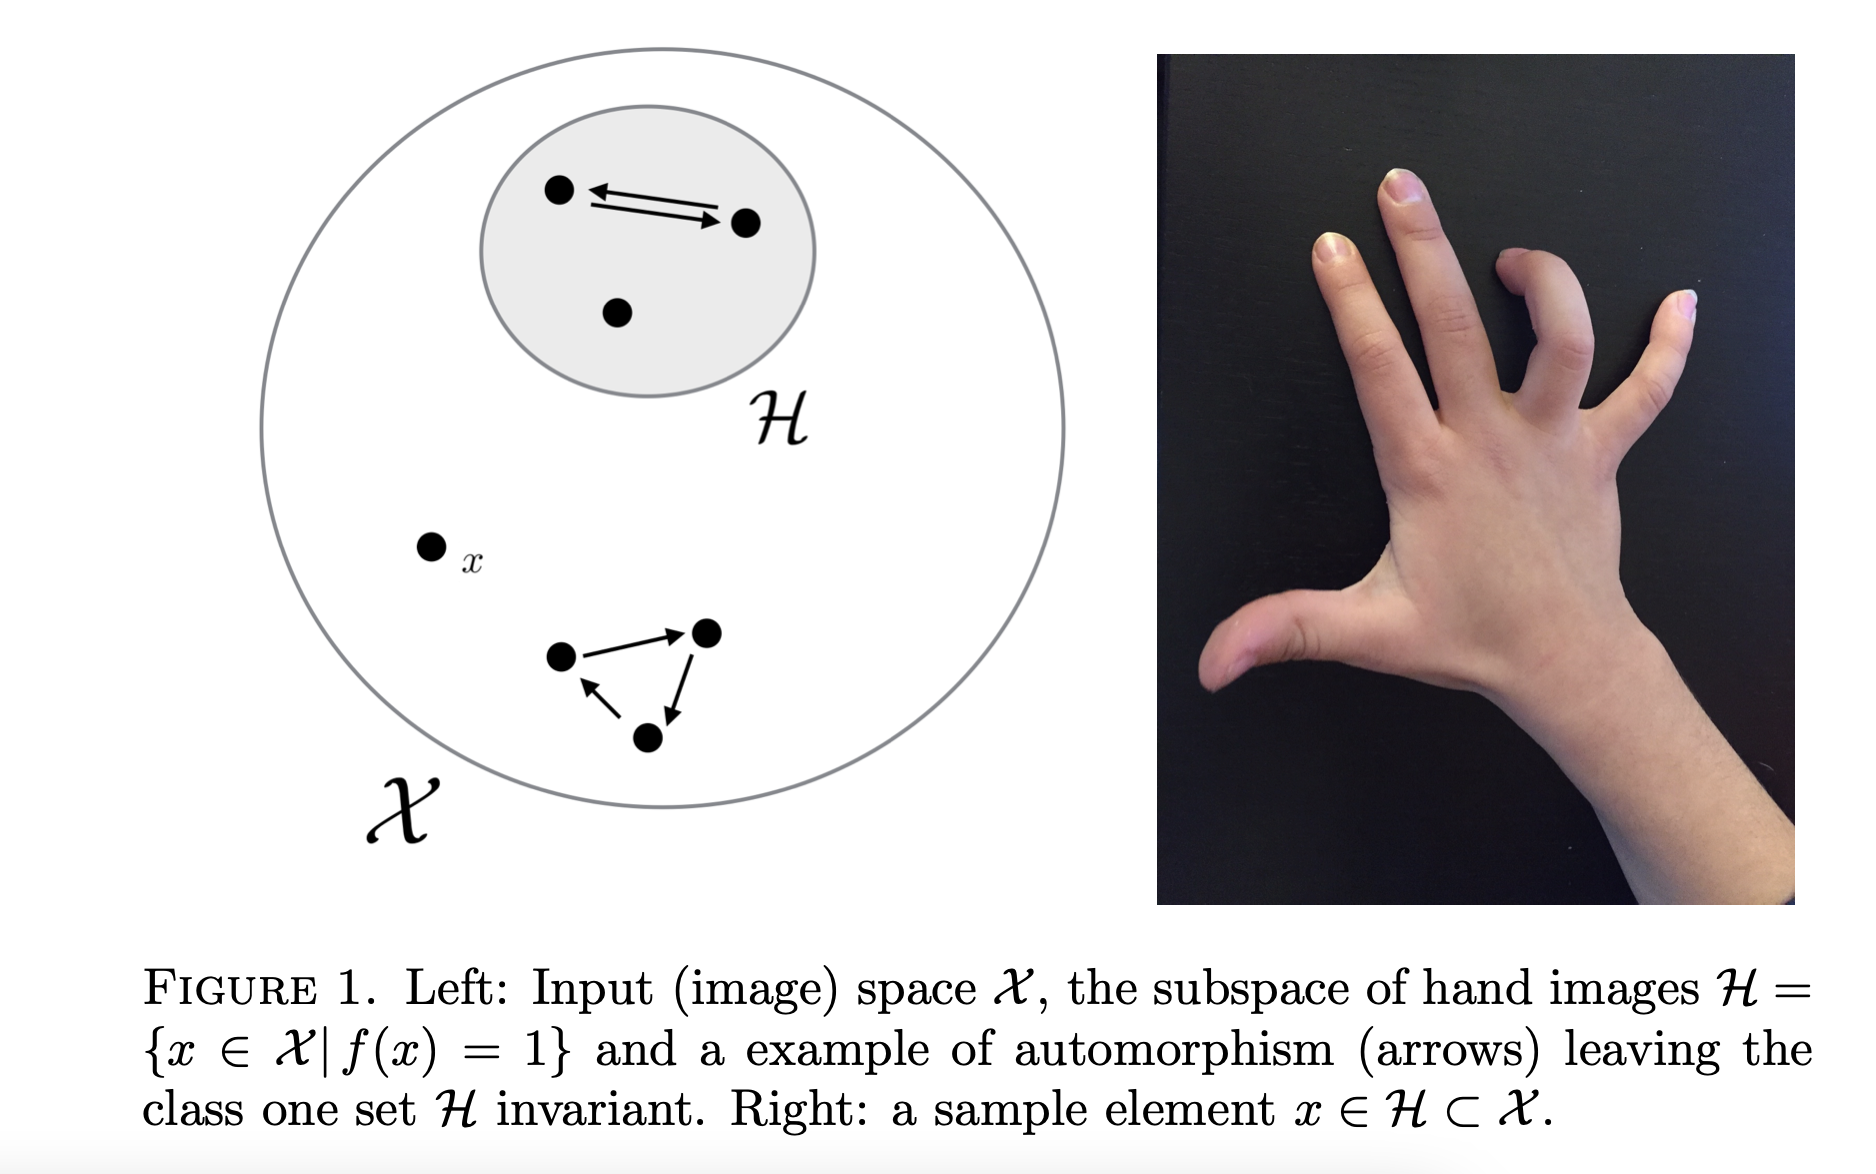
\includegraphics[height=4cm]{img/hand2.png}
  \end{center}
  
Suppose we are given a stack of images of a hand, e.g., from the frames of a movie of a moving hand created using a generating function,
$y = f(\theta)$, where $y$ is the image in a frame and $\theta$ a parametrization of the hand image and view.
\end{frame}

\begin{frame}[label=ladila]{Model III}
 \begin{center}%\includegraphics[height=1.2cm]{COPL}%
  %\hspace{2cm}
  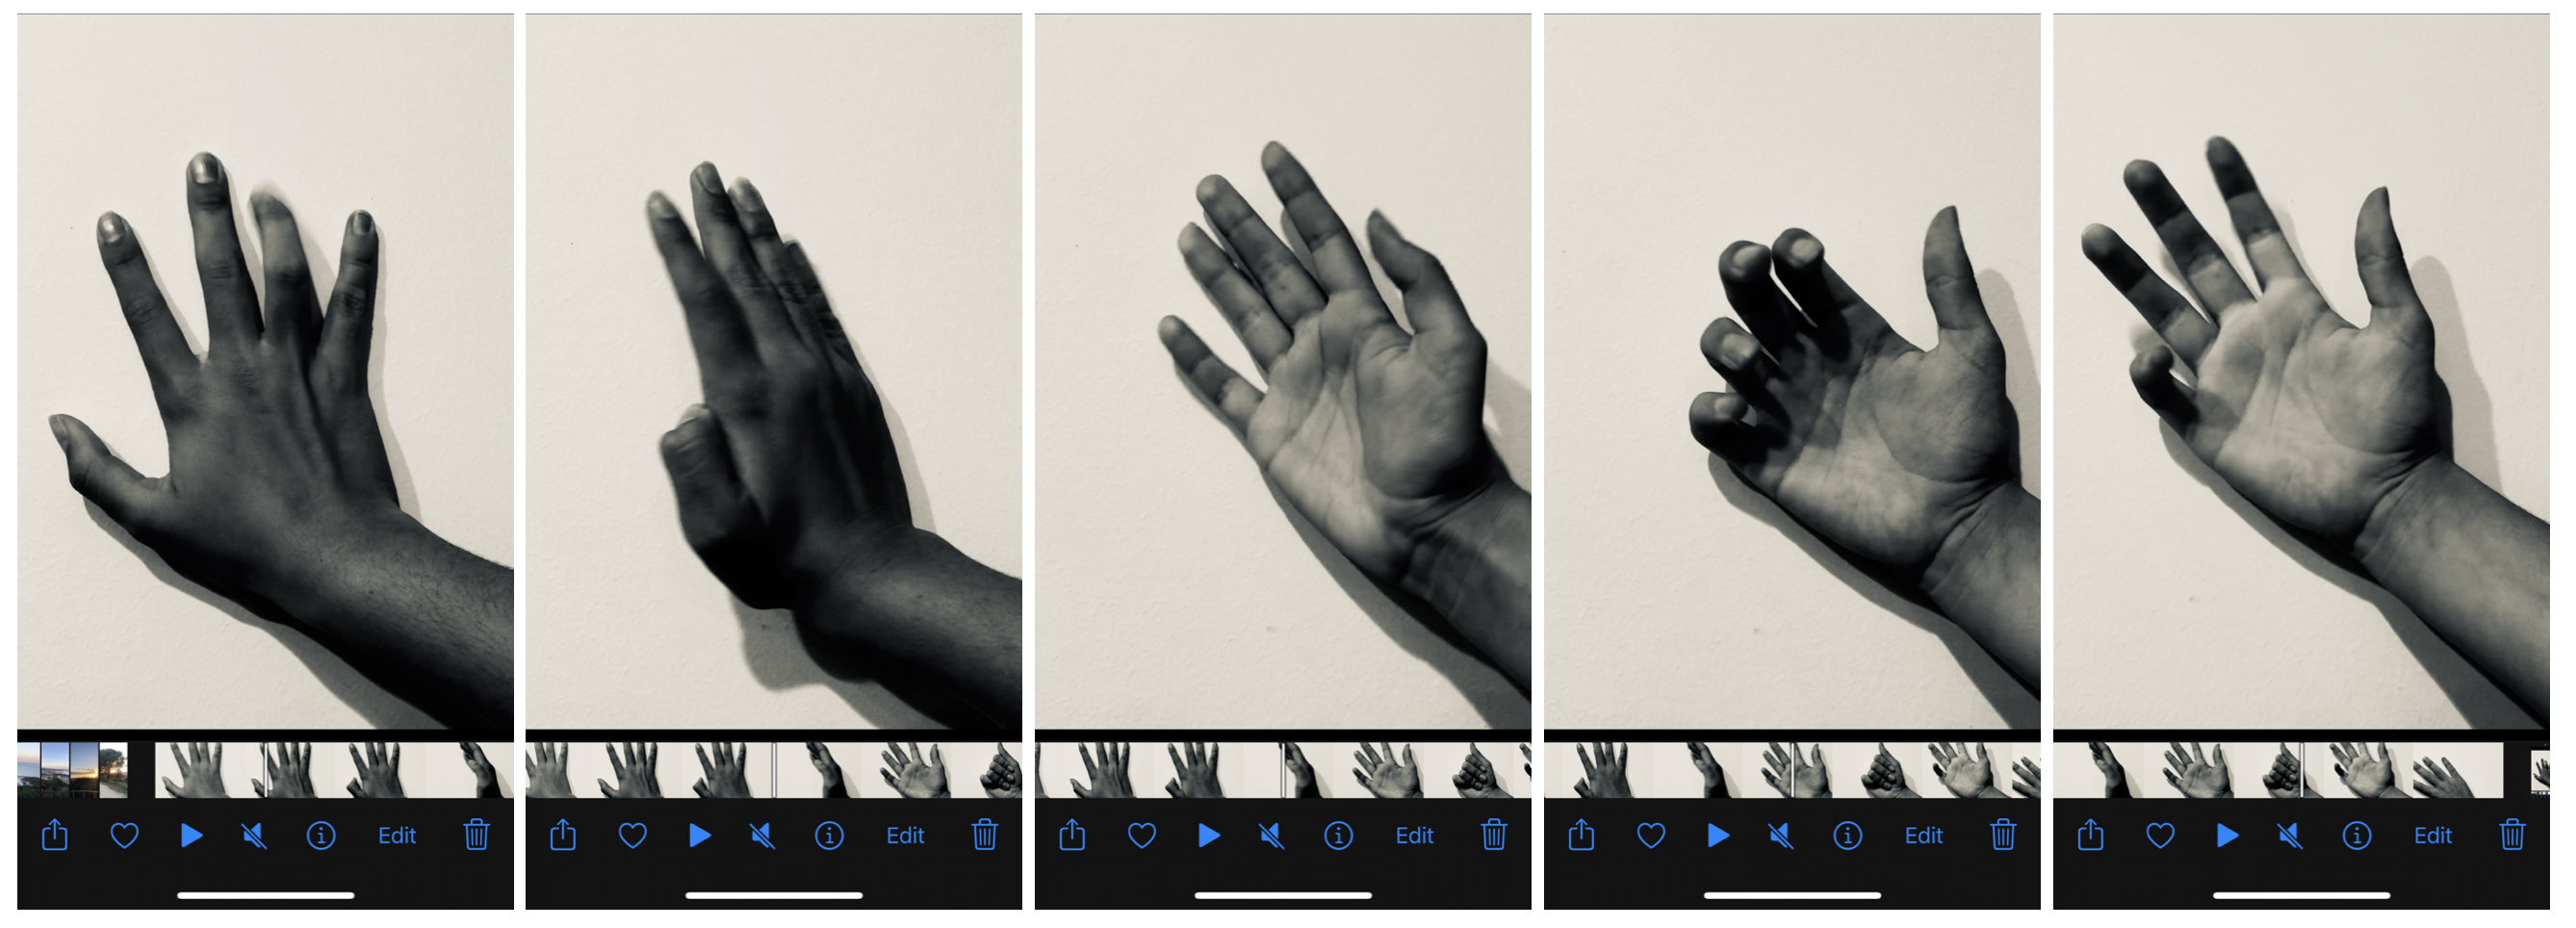
\includegraphics[height=5cm]{img/hands.png}
  \end{center}
  The structure of the dataset is encapsulated by the minimal program that encodes the function $y=f(x)$---the {\em invariant} object.  %The {\bf symmetries} of the dataset are parametrized by $\theta$, and they are symmetries in the sense that if $\theta\rightarrow \theta'$ and $y\rightarrow y'$, then the equation $y'-f(\theta') =0 $ holds true.
\end{frame}



%%%%%%%%%%%%%%%%%%%%%%%%%%%%%%%%%%%%%%%%%%%%%%%%%%%%%%%%%%%%%%%%%%%%%%
\begin{frame}[label=ladila]{Why are ``good models'' good?}

The rationale for the importance of compressive (succinct) models is discussed in detail in \cite{Ruffini:2007aa,Ruffini:2009aa,Ruffini2017}.  Rephrase of the principle of Occam’s Razor: {\em
one should not increase, beyond what is necessary, the number of entities required to explain anything.}  Ok, but why? Options:\vfill

a) The universe appears to be simple. Simple rules can create apparent complexity.\vfill


b) Simple data generators are more likely if the universe rules are drawn from a random algorithmic bingo (Solomonoff's prior). \vfill

% c) Simple models are unbiased and generalize better (Occam, Laplace, Jaynes). \vfill

d) Natural selection A: they are easier to construct,  store,  and reuse for model-building. \vfill

e) Natural selection B: favors agents that coarse grain the world in a way that can be modeled simply. This motivates a definition of \textbf{Emergence}.

%Simple models can be maximally powerful (Turing complete)

\end{frame}

\begin{frame}[label=emergence]{From the algorithmic agent to emergence}
Find patterns and operate at some coarse-graining level for survival \cite{ruffiniNavigatingComplexityHow2024}.

\begin{definition}
  \textbf{Emergence} occurs when the coarse-graining of a complex system transforms data that appears incompressible (with high apparent Kolmogorov complexity and high entropy) at the microscopic level into a new system that retains non-trivial structure (high entropy) but can be compressed by a simpler, lower-complexity model.  
\end{definition}

\begin{center}%\includegraphics[height=1.2cm]{COPL}%
  %\hspace{2cm}
  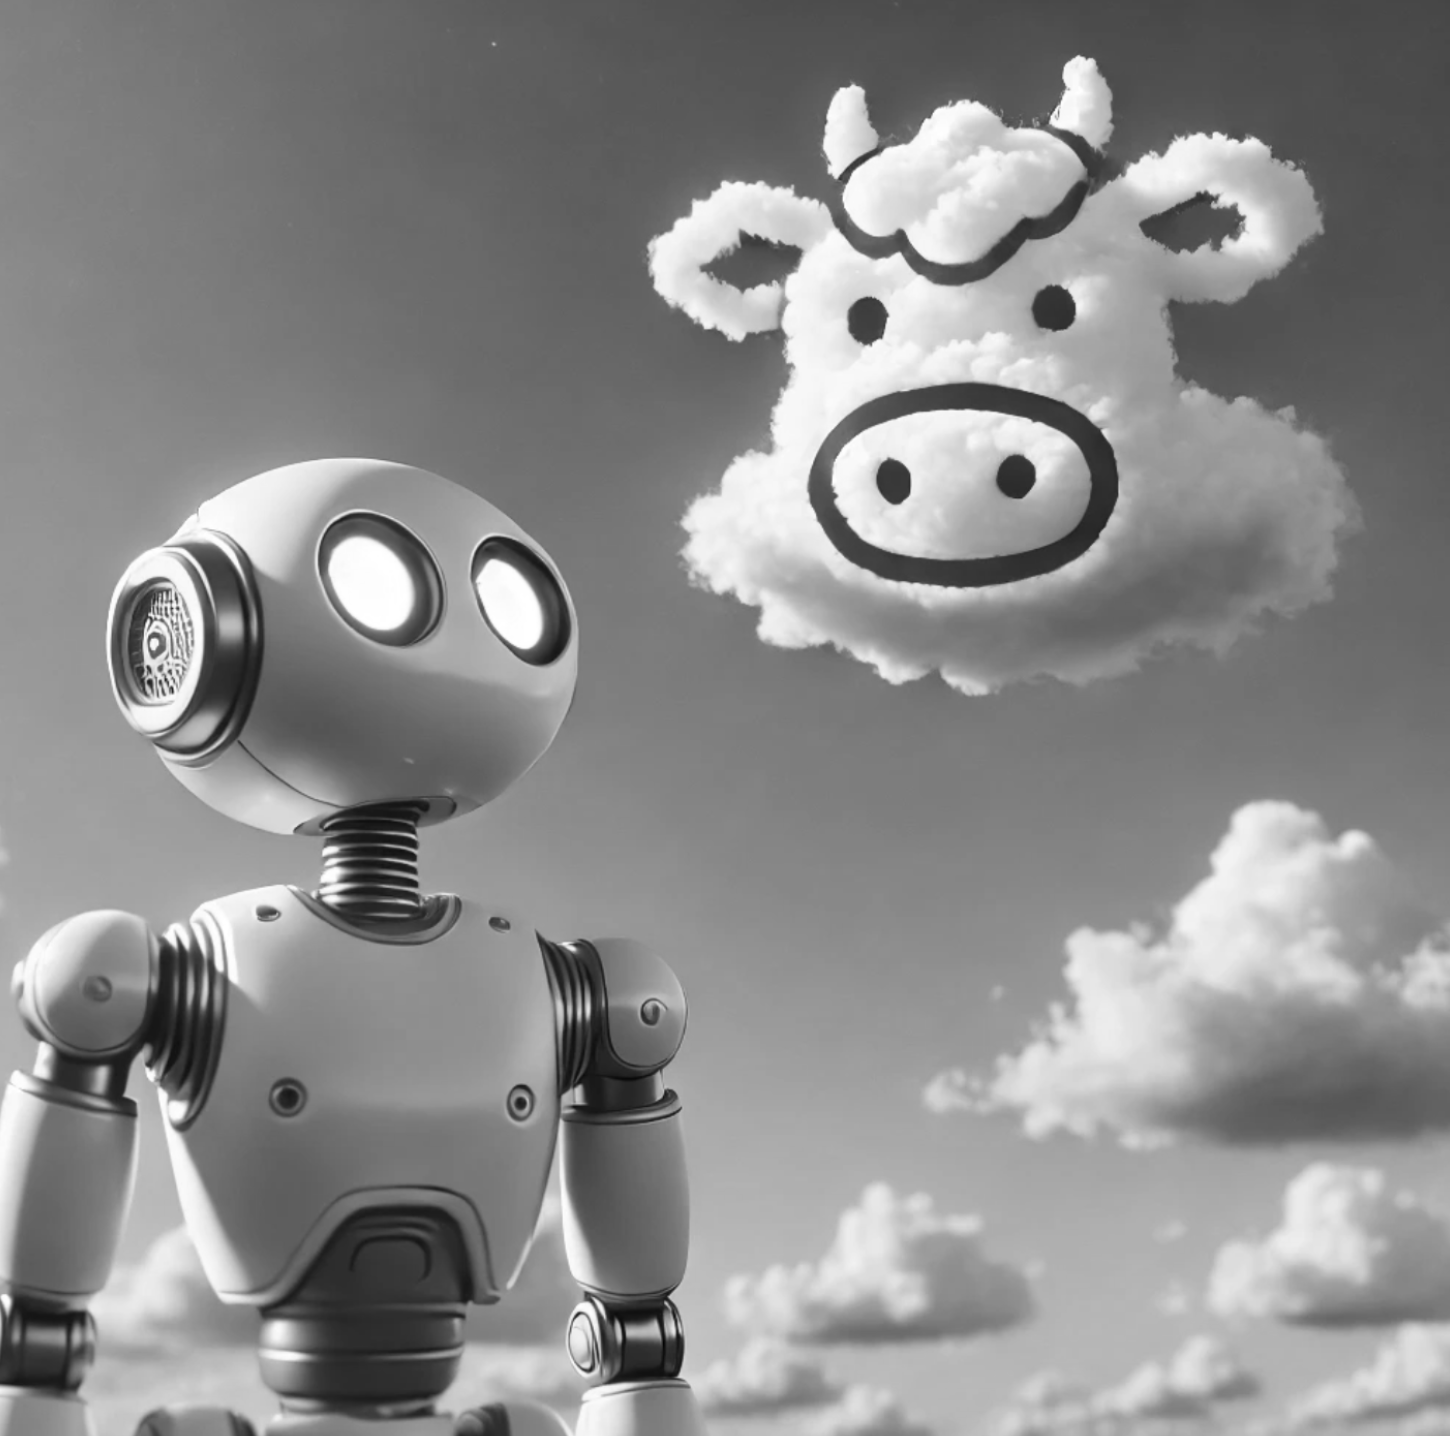
\includegraphics[height=3cm]{img/robot_emergence.png}
  \end{center}

\end{frame}

\begin{frame}[label=bayesian]{From the algorithmic agent to Bayesian inference I}
Bayesian inference naturally arises as agents strive for efficient prediction and compression \cite{ruffiniNavigatingComplexityHow2024}.

This  links KT  with theories such as Karl Friston's Free Energy Principle, and Active Inference \cite{parr2022active}. \ \\ 

%Consider an Agent tasked with compressing random pages from the Library of Congress ``on the fly".  %They arrive in some unknown order, and K must choose a model after the first few lines of text.


\begin{center}%\includegraphics[height=1.2cm]{COPL}%
  %\hspace{2cm}
  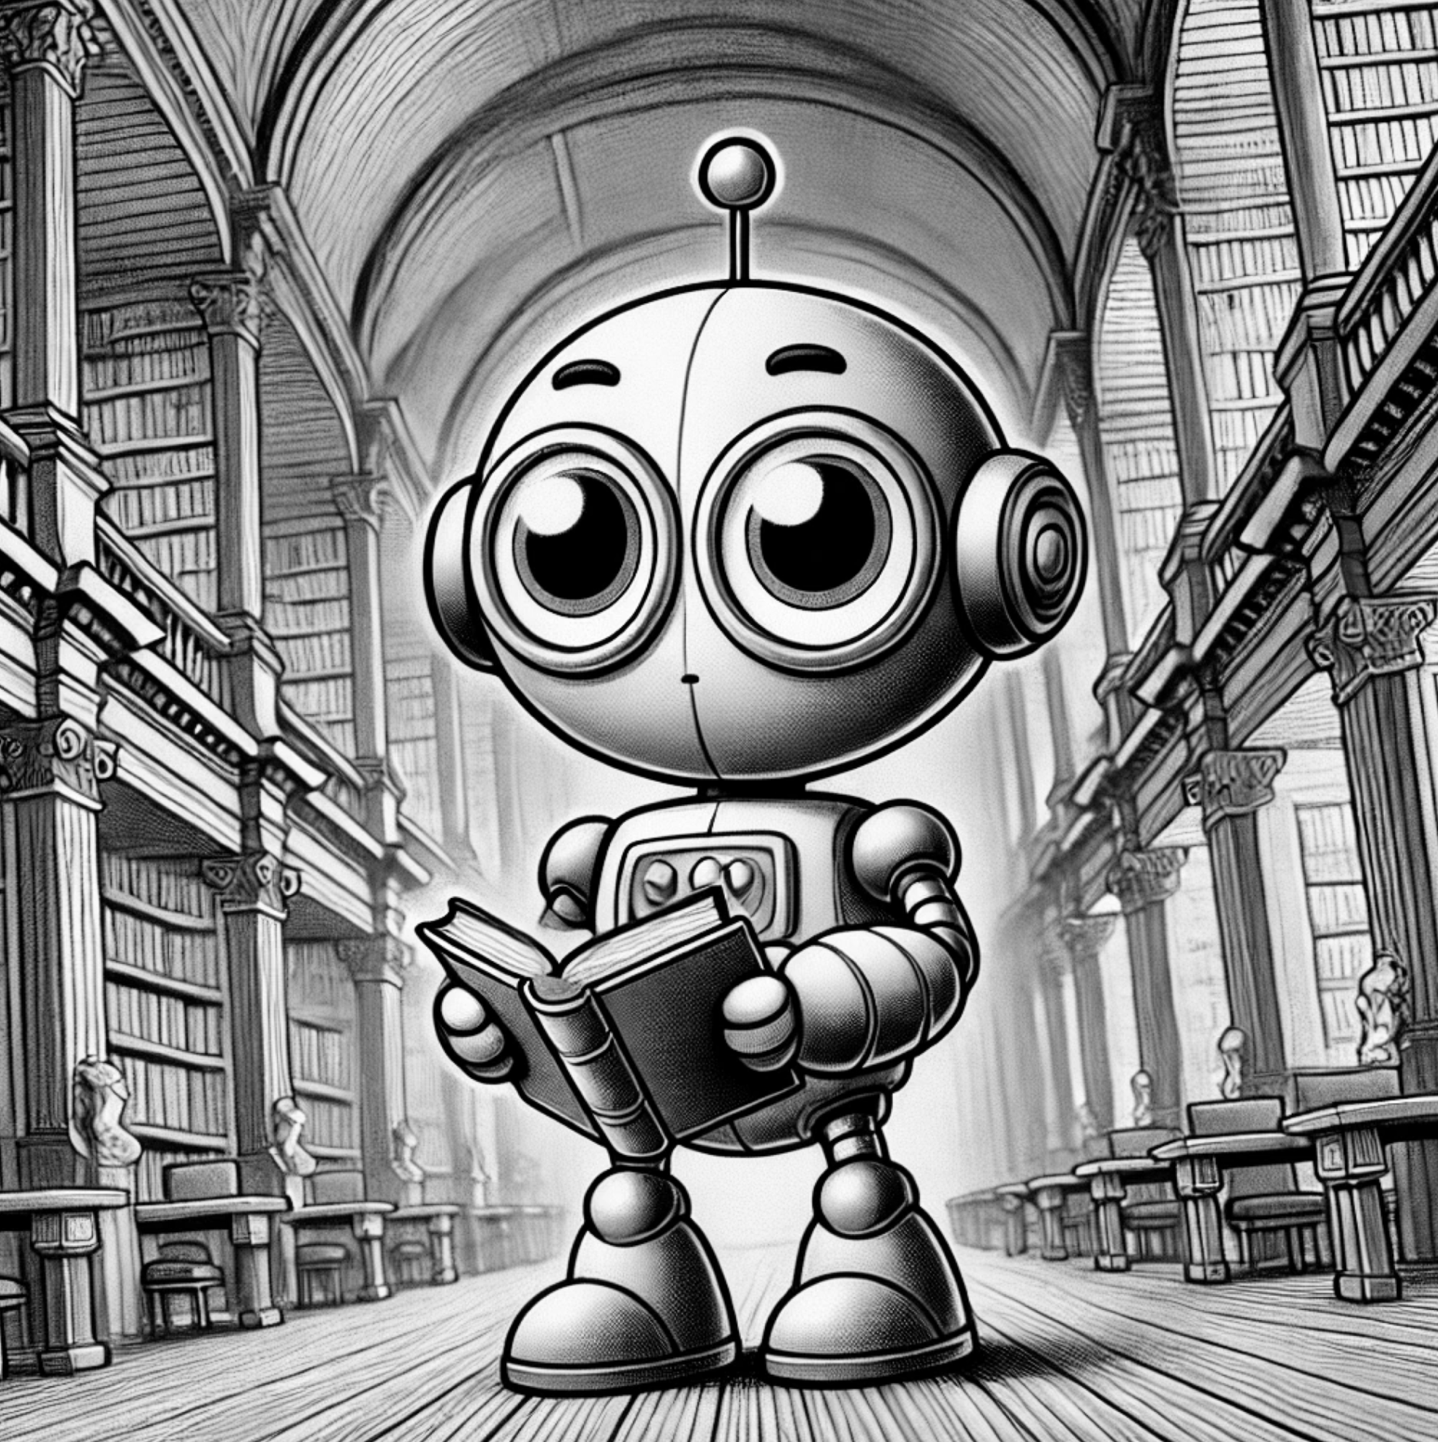
\includegraphics[height=3cm]{img/robot_library.png}
  \end{center}
  
% Task challenges: a) \textbf{partial access to data} from the world, sequential data arrival: the agent receives one page at a time and must update its model as it encounters new content; b)  \textbf{diversity of content}: the library contains various types of documents in different languages, such as novels, research papers, and poetry, each with different structures and linguistic patterns; c) need to act



\end{frame}

% \begin{frame}[label=bayesian]{From the algorithmic agent to Bayesian inference II}
% \textbf{Compression strategy:} Maintain multiple submodels, each optimized for different content types (e.g., one for English fiction, another for academic writing in Italian).

% \textbf{Model selection:} The agent selects the most appropriate model for each incoming page based on the likelihood or probability of relevance and prior experiences.

% \textbf{Posterior optimization:} Models frequently observed in past data can use more compressive schemes, while rarer models are less favored (similar to Huffman coding).

% %This is essentially a route to Bayesian inference.



% \end{frame}


% \begin{frame}[label=bayesian1]{From Algorithmic Agents to Bayesian Inference I}
% \textbf{Agent's Task:} Compress data \emph{on the fly}, where data is sequentially fed from multiple submodels chosen randomly.  

% \vspace{1em}

% \textbf{Objective:} Achieve optimal compression at each step; success is measured by the cumulative compression achieved.

% \vspace{1em}

% \textbf{Challenges:}
% \begin{itemize}
%     \item \textbf{Uncertainty of Data Source:} Each data point originates from an unknown submodel.
%     \item \textbf{Immediate Action Required:} Must update and select the compression model at each step.
%     \item \textbf{Retrospective Analysis Allowed:} Can analyze all past observed data to improve future compression.
% \end{itemize}
% \end{frame}

% \begin{frame}[label=bayesian2]{From Algorithmic Agents to Bayesian Inference II}
% \textbf{Necessity of Probabilistic Modeling:}
% \begin{itemize}
%     \item \textbf{Use of Past Frequencies:} Past observed frequencies of submodels form empirical priors.
%     \item \textbf{Probabilistic Framework:} Estimate the probability of each submodel generating the next data point.
% \end{itemize}

% \vspace{1em}

% \textbf{Bayesian Updating:}
% \[
% P(M_i | D_{1:t}) = \frac{P(D_t | M_i) \, P(M_i | D_{1:t-1})}{\sum_j P(D_t | M_j) \, P(M_j | D_{1:t-1})}
% \]
% \begin{itemize}
%     \item \( P(M_i | D_{1:t-1}) \): Prior probability of submodel \( M_i \) based on past data.
%     \item \( P(D_t | M_i) \): Likelihood of new data \( D_t \) given submodel \( M_i \).
%     \item \textbf{Posterior Probability:} Guides model selection for optimal compression.
% \end{itemize}
% \end{frame}


% \begin{frame}[label=bayesian3]{From Algorithmic Agents to Bayesian Inference III}
% \textbf{Compression Efficiency and Probabilities:}
% \begin{itemize}
%     \item \textbf{Shannon's Source Coding Theorem:} Optimal code length is \( L(D_t | M_i) = -\log P(D_t | M_i) \).
%     \item \textbf{AIT Connection:} Shorter descriptions correspond to higher probability models.
% \end{itemize}

% \vspace{1em}

% \textbf{Conclusion:}
% \begin{itemize}
%     \item The agent's task and constraints give rise to probabilistic reasoning.
%     \item \textbf{Bayesian Inference Emerges Naturally:} Updating model probabilities based on observed data aligns with Bayesian principles.
%     %\item \textbf{Optimal Compression Achieved:} By continuously refining model probabilities, the agent minimizes code lengths over time.
% \end{itemize}
% \end{frame}

% \begin{frame}[label=bayesian1]{From Algorithmic Agents to Bayesian Inference I}
% \textbf{Agent's Task:} Compress data \emph{on the fly}, where data is sequentially fed from multiple submodels chosen randomly.

% \vspace{1em}

% \textbf{Objective:} Achieve optimal compression at each step; success is measured by the cumulative compression achieved.

% \vspace{1em}

% \textbf{Agent's Capabilities:}
% \begin{itemize}
%     \item Access to different computational models (programs) suitable for various types of data.
%     \item Ability to select and switch between models based on observed data.
%     \item Retrospective analysis of all past observed data to inform model selection.
% \end{itemize}
% \end{frame}

% \begin{frame}[label=bayesian2]{From Algorithmic Agents to Bayesian Inference II}
% \textbf{Challenge of Model Selection:}
% \begin{itemize}
%     \item \textbf{Uncertainty of Data Source:} Each data point originates from an unknown submodel.
%     \item \textbf{Trade-off in Model Choice:}
%     \begin{itemize}
%         \item Some models are shorter (simpler) but may compress data less effectively.
%         \item Other models are longer (more complex) but offer better compression if correctly matched.
%     \end{itemize}
%     \item \textbf{Risk of Model Errors:}
%     \begin{itemize}
%         \item Choosing an incorrect model leads to compression errors.
%         \item Errors must be stored or corrected, impacting overall compression efficiency.
%     \end{itemize}
% \end{itemize}

% \vspace{1em}

% \textbf{Need for Probabilistic Strategy:}
% \begin{itemize}
%     \item Use past observed frequencies of models to estimate their likelihood.
%     \item Balance between model complexity and expected compression gain.
% \end{itemize}
% \end{frame}

% \begin{frame}[label=bayesian3]{From Algorithmic Agents to Bayesian Inference III}
% \textbf{Bayesian Inference Emergence:}
% \begin{itemize}
%     \item \textbf{Prior Probabilities:} Based on past frequency of models.
%     \item \textbf{Likelihood:} How well each model fits (compresses) the new data.
%     \item \textbf{Posterior Probabilities:} Update beliefs about models after observing new data.
% \end{itemize}

% \vspace{1em}

% \textbf{Agent's Decision Strategy:}
% \begin{itemize}
%     \item Select the model that maximizes expected compression efficiency.
%     \item Consider both the probability of the model and its potential compression rate.
%     \item Account for the cost of errors if the model is incorrect.
% \end{itemize}

% \vspace{1em}

% \textbf{Conclusion:}
% \begin{itemize}
%     \item \textbf{Bayesian Inference Naturally Arises:} The agent uses a Bayesian approach to balance trade-offs in model selection.
%    % \item \textbf{Optimal Compression Achieved:} By updating model probabilities and considering potential risks, the agent minimizes overall code length.
%     %\item \textbf{AIT Connection:} The pursuit of the shortest effective program leads to probabilistic reasoning when faced with uncertainty.
% \end{itemize}
% \end{frame}

\begin{frame}{Agenthood and the Emergence of Probability}
\begin{itemize}
    \item \textbf{Thesis}: Probability and Bayesian inference are consequences of agenthood within Algorithmic Information Theory (AIT).
    \item Agents seek to \textbf{predict the world efficiently} by finding \textbf{short codes} for data (Solomonoff/Occam).
    \item \textbf{Agent Limitations}:
    \begin{itemize}
        \item Computational constraints.
        \item Partial access to data (\textit{coarse-grained} observations).
        \item Dealing with \textit{noisy} and \textit{incomplete} data.
    \end{itemize}
\end{itemize}
\end{frame}

\begin{frame}{From Compression to Bayesian Methods}
\begin{itemize}
    \item \textbf{Noisy Data} $\Rightarrow$ \textbf{Shannon's Information Theory}
    \begin{itemize}
        \item Noise introduces uncertainty.
        \item Efficient compression requires probabilistic encoding.
    \end{itemize}
    \item \textbf{Incomplete Data and Coarse-Graining}
    \begin{itemize}
        \item Limited observations lead to incomplete data.
        \item Coarse-graining aggregates data, losing fine details.
        \item Both necessitate probabilistic models to capture uncertainty.
    \end{itemize}
    \item \textbf{Computational Limitations}
    \begin{itemize}
        \item Uncomputability of Kolmogorov complexity ($K$).
        \item Agents approximate $K$ using probabilistic methods.
    \end{itemize}
\end{itemize}
\end{frame}

% \begin{frame}{Emergence of Bayesian Inference}
% \begin{itemize}
%     \item \textbf{Agents Develop Bayesian Methods}:
%     \begin{itemize}
%         \item To update beliefs based on new data.
%         \item To manage uncertainty in predictions.
%     \end{itemize}
%     \item \textbf{Compression and Probability}
%     \begin{itemize}
%         \item Shortest codes achieved by modeling data distributions.
%         \item Probability distributions optimize compression under constraints.
%     \end{itemize}
%     \item \textbf{Conclusion}:
%     \begin{itemize}
%         \item Bayesian inference naturally arises as agents strive for efficient prediction and compression.
%         \item Agent limitations and data characteristics lead to the adoption of probabilistic frameworks.
%     \end{itemize}
% \end{itemize}
% \end{frame}